\documentclass[12pt]{article}

\usepackage{amsmath,amsthm,amsfonts,amssymb,amsxtra}
\usepackage{pgf,tikz}
\usetikzlibrary{arrows}
\renewcommand{\theenumi}{(\alph{enumi})} 
\renewcommand{\labelenumi}{\theenumi}

\pagestyle{empty}
\setlength{\textwidth}{7in}
\setlength{\oddsidemargin}{-0.5in}
\setlength{\topmargin}{-1.0in}
\setlength{\textheight}{9.5in}

\newtheorem{problem}{Problem}

\begin{document}

%%%%%%%%%%%%%%%%%%%%%%%%%%%%%%%%%%%%% Page 1
\noindent{\large\bf MATH 141}\hfill{\large\bf Final Exam---Practice Test.}\hfill{\large\bf
  Fall 2009}\hfill{\large\bf Page 1/10}\hrule

\bigskip
{\problem[50 pts] \em Compute the following limits:}

\bigskip
\noindent
\begin{tikzpicture}
\draw (4cm,14cm) node{
(a) $\displaystyle{\lim_{x \to 3} \frac{x^2-2x}{x+1}} = \mbox{}$ };
\draw (6cm,13.4cm) rectangle (11cm,14.6cm);
\draw (4cm, 10cm) node{
(b) $\displaystyle{\lim_{x \to \infty} \Big( 1 + \frac{5}{x} \Big)^{3x}} = \mbox{}$}; 
\draw (6cm,9.4cm) rectangle (11cm,10.6cm);
\draw (4cm, 6cm) node{
(c) $\displaystyle{\lim_{x \to -\infty} \sqrt{5-x}} = \mbox{}$};
\draw (6cm,5.4cm) rectangle (11cm,6.6cm);
\draw (4cm, 2cm) node{
(d) $\displaystyle{\lim_{x \to \infty} \frac{5x^2+7}{3x^2-x}} = \mbox{}$};
\draw (6cm, 1.4cm) rectangle (11cm,2.6cm);
\draw (4cm, -2cm) node{
(e) $\displaystyle{\lim_{x\to 0} \frac{e^x-1}{\tan x}} = \mbox{}$}; 
\draw (6cm, -2.6cm) rectangle (11cm,-1.4cm);
\end{tikzpicture}
\newpage
%%%%%%%%%%%%%%%%%%%%%%%%%%%%%%%%%%%%% Page 2
\noindent{\large\bf MATH 141}\hfill{\large\bf Final Exam---Practice Test.}\hfill{\large\bf
  Fall 2009}\hfill{\large\bf Page 2/10}\hrule

\bigskip
{\problem[50 pts] \em Find the derivative of the following functions:}
\begin{enumerate}
\item $\displaystyle{y = \frac{x^3 + x^2 + x - 1}{x^{3/2}}}$.
\begin{flushright}
  \begin{tikzpicture}
    \draw (-1cm,0.5cm) node {$\displaystyle{\frac{dy}{dx}} = $};
    \draw (0cm,-0.2cm) rectangle (5cm,1.2cm);
  \end{tikzpicture}
\end{flushright}
\item $f(x) = \cos^2 (e^x) + \sin^2 (e^x)$.
\begin{flushright}
  \begin{tikzpicture}
    \draw (-1cm,0.5cm) node {$f'(x) = $};
    \draw (0cm,-0.2cm) rectangle (5cm,1.2cm);
  \end{tikzpicture}
\end{flushright}
\item $f(x) = e^{9x+3}$
\vspace{1cm}
\begin{flushright}
  \begin{tikzpicture}
    \draw (-1cm,0.5cm) node {$f'(x) = $};
    \draw (0cm,-0.2cm) rectangle (5cm,1.2cm);
  \end{tikzpicture}
\end{flushright}
\item $g(t) = \ln \big( \sin^{-1}(t) \big)$. \textbf{Hint: } $\displaystyle{ \frac{d}{dx} \big( \sin^{-1} y \big) = \frac{1}{\sqrt{1-y^2}} \frac{dy}{dx}} $.
\vspace{2cm}
\begin{flushright}
  \begin{tikzpicture}
    \draw (-1cm,0.5cm) node {$g'(t) = $};
    \draw (0cm,-0.2cm) rectangle (5cm,1.2cm);
  \end{tikzpicture}
\end{flushright}
\item $f(x) = \displaystyle{\frac{\sec x + x^{-2}}{x^{-2}\sec x}}$.
\vspace{2cm}
\begin{flushright}
  \begin{tikzpicture}
    \draw (-1cm,0.5cm) node {$f'(x) = $};
    \draw (0cm,-0.2cm) rectangle (5cm,1.2cm);
  \end{tikzpicture}
\end{flushright}
\end{enumerate}
\newpage

%%%%%%%%%%%%%%%%%%%%%%%%%%%%%%%%%%%%% Page 3
\noindent{\large\bf MATH 141}\hfill{\large\bf Final Exam---Practice Test.}\hfill{\large\bf
  Fall 2009}\hfill{\large\bf Page 3/10}\hrule

\bigskip
{\problem[50 pts] \em  Evaluate each integral:} 

\bigskip
\begin{tikzpicture}
\draw (4cm,14cm) node[left, text width=6.5cm]{
(a) $\displaystyle{\int \big( x^{2} + \frac{2}{x} - e^{x-1} \big)\, dx} = \mbox{}$ };
\draw (2.5cm,13.4cm) rectangle (9cm,14.6cm);
\draw (4cm, 11cm) node[left, text width=6.5cm]{
(b) $\displaystyle{\int_0^{\pi/4} \big( 3\sec^2 x - 2\cos^2 x \big)\, dx} = \mbox{}$}; 
\draw (3.75cm,10.4cm) rectangle (9cm,11.6cm);
\draw (4cm, 8cm) node[left, text width=6.5cm]{
(c) $\displaystyle{\int ( 3 + \sin t)^{3} \cos t\, dt} = \mbox{}$}; 
\draw (2.5cm,7.4cm) rectangle (9cm,8.6cm);
\draw (4cm, 4cm) node[left, text width=6.5cm]{
(d) $\displaystyle{\int \frac{3x^2}{(x^3-3)^3}\, dx} = \mbox{}$}; 
\draw (1.5cm, 3.4cm) rectangle (9cm,4.6cm);
\draw (4cm, 0cm) node[left, text width=6.5cm]{
(e) $\displaystyle{\int_0^2 x \sin(x^2)\, dx} = \mbox{}$};
\draw (1.5cm, -0.4cm) rectangle (9cm,0.6cm);
\end{tikzpicture}
\newpage

%%%%%%%%%%%%%%%%%%%%%%%%%%%%%%%%%%%%% Page 4
\noindent{\large\bf MATH 141}\hfill{\large\bf Final Exam---Practice Test.}\hfill{\large\bf
  Fall 2009}\hfill{\large\bf Page 4/10}\hrule
  
\bigskip
{\problem[50 pts] \em Let $f(x) = \displaystyle{\frac{3(x+1)(x-3)}{(x+2)(x-4)}}$. Given that}
\begin{equation*}
f'(x) = \frac{-30(x-1)}{(x+2)^2(x-4)^2}, \text{and } f''(x) =\frac{90(x^2-2x+4)}{(x+2)^2(x-4)^3}, 
\end{equation*}
sketch the graph of $f$ (in the next page), and determine the following properties:

\bigskip
\begin{tikzpicture}
\draw (4cm,14cm) node[left, text width=10cm]{
(a) The $x$- and $y$-intercepts are};
\draw (-0.25cm,13.4cm) rectangle (9cm,14.6cm);
\draw (4cm, 12cm) node[left, text width=10cm]{
(b) The vertical asymptotes are }; 
\draw (-0.25cm,11.4cm) rectangle (9cm,12.6cm);
\draw (4cm, 10cm) node[left, text width=10cm]{
(c) The horizontal asymptote is}; 
\draw (-0.25cm,9.4cm) rectangle (9cm,10.6cm);
\draw (4cm, 8cm) node[left, text width=10cm]{
(d) The graph is above the $x$-axis on the intervals}; 
\draw (-2cm, 6.4cm) rectangle (9cm,7.6cm);
\draw (4cm, 6cm) node[left, text width=10cm]{
(e) The graph is increasing on the intervals}; 
\draw (-2cm, 4.4cm) rectangle (9cm,5.6cm);
\draw (4cm, 4cm) node[left, text width=10cm]{
(f) The graph is decreasing on the intervals}; 
\draw (-2cm, 2.4cm) rectangle (9cm,3.6cm);
\draw (4cm, 2cm) node[left, text width=10cm]{
(g) The graph is concave-up on the intervals}; 
\draw (-2cm, 0.4cm) rectangle (9cm,1.6cm);
\draw (4cm, 0cm) node[left, text width=10cm]{
(h) The graph is concave-down on the intervals}; 
\draw (-2cm, -1.6cm) rectangle (9cm,-0.4cm);
\draw (4cm, -2.5cm) node[left, text width=10cm]{
(i) A relative maximum point on the graph is};
\draw (2.5cm,-3.1cm) rectangle (9cm,-1.9cm);
\draw (2cm, -4cm) node[draw, text width=0.7\linewidth, text justified, rounded corners]{
{\em Use the next page for scratch.  Support your claims with sign-charts.}
};
\end{tikzpicture}
\newpage
%%%%%%%%%%%%%%%%%%%%%%%%%%%%%%%%%%%%% Page 5
\noindent{\large\bf MATH 141}\hfill{\large\bf Final Exam---Practice Test.}\hfill{\large\bf
  Fall 2009}\hfill{\large\bf Page 5/10}\hrule

\bigskip
\begin{center}
\begin{tikzpicture}
\begin{scope}[scale=1.25]
\clip (0cm, 0cm) rectangle (10cm,10cm);
\begin{scope}[xshift=5cm, yshift=5cm]
\draw[gray, very thin, step=0.5cm] (-4.4cm,-4.4cm) grid (4.4cm, 4.4cm);
\draw[<->, very thick] (0cm, -5cm) -- (0cm, 5cm);
\draw[<->, very thick] (-5cm, 0cm) -- (5cm, 0cm);
\end{scope}
\end{scope}
\end{tikzpicture}
\end{center}  
\newpage


%%%%%%%%%%%%%%%%%%%%%%%%%%%%%%%%%%%%% Page 6
\noindent{\large\bf MATH 141}\hfill{\large\bf Final Exam---Practice Test.}\hfill{\large\bf
  Fall 2009}\hfill{\large\bf Page 6/10}\hrule

\bigskip
{\problem[10 pts] \em  Find the natural domain of the function $f(x) = \sqrt{x^2-2x+5}$.}
\begin{enumerate}
\item All reals.
\item $x < 5$
\item $x \geq 5$
\item $x \neq 5$
\item $x^2-2x \neq 5$
\end{enumerate}
\vspace{1cm}
\hrule
{\problem[10pts] \em Express $f(x) = \lvert x^2-3x+5 \rvert$ as a composition of two functions; that is, find $g$ and $h$ such that $f= g \circ h$.}
\vspace{1cm}
\begin{flushright}
  \begin{tikzpicture}
    \draw (-0.5cm,0.5cm) node {$h =$};
    \draw (0cm,0cm) rectangle (5cm,1.2cm);
    \draw (-0.5cm,2cm) node {$g =$};
    \draw (0cm,1.4cm) rectangle (5cm,2.6cm);
  \end{tikzpicture}
\end{flushright}
\hrule
{\problem[10pts] \em Find the amplitude and period of}
\begin{equation*}
y = 5 \cos( 2x + \pi).
\end{equation*}
\vspace{0.5cm}
\begin{flushright}
  \begin{tikzpicture}
    \draw (-1.25cm,0.5cm) node {$\text{Amplitude} =$};
    \draw (0cm,0cm) rectangle (5cm,1.2cm);
    \draw (-1cm,2cm) node {$\text{period} =$};
    \draw (0cm,1.4cm) rectangle (5cm,2.6cm);
  \end{tikzpicture}
\end{flushright}
\hrule
{\problem[10 pts] \em Solve for $x$:}
\begin{equation*}
\log x^2 + \log x = 30.
\end{equation*}
\vspace{2cm}
\begin{flushright}
  \begin{tikzpicture}
    \draw (-0.5cm,0.5cm) node {$x =$};
    \draw (0cm,0cm) rectangle (5cm,1.2cm);
  \end{tikzpicture}
\end{flushright}
\newpage

%%%%%%%%%%%%%%%%%%%%%%%%%%%%%%%%%%%%% Page 7
\noindent{\large\bf MATH 141}\hfill{\large\bf Final Exam---Practice Test.}\hfill{\large\bf
  Fall 2009}\hfill{\large\bf Page 7/10}\hrule
  
\bigskip
{\problem[10 pts] Sketch the curve by eliminating the parameter (i.e.~try to write $y=f(x)$.) Label the axes accordingly.}
\begin{equation*}
x=3t-1,\quad y=6t+2.
\end{equation*}
\begin{flushright}
\begin{tikzpicture}
\begin{scope}[scale=0.75]
\clip (0cm, 0cm) rectangle (10cm,10cm);
\begin{scope}[xshift=5cm, yshift=5cm]
\draw[gray, very thin, step=0.5cm] (-4.4cm,-4.4cm) grid (4.4cm, 4.4cm);
\draw[<->, very thick] (0cm, -5cm) -- (0cm, 5cm);
\draw[<->, very thick] (-5cm, 0cm) -- (5cm, 0cm);
\end{scope}
\end{scope}
\end{tikzpicture}
\end{flushright}
\hrule
{\problem[10 pts] \em Find the value of the constant $k$ for which the following function is continuous everywhere:}
\begin{equation*}
f(x) = \begin{cases}
7x-2 &\text{if }x \leq 1, \\
kx^2 &\text{if }x < 1.
\end{cases}
\end{equation*}
\begin{flushright}
  \begin{tikzpicture}
    \draw (-0.5cm,0.5cm) node {$k =$};
    \draw (0cm,0cm) rectangle (5cm,1.2cm);
  \end{tikzpicture}
\end{flushright}
\hrule
{\problem[10 pts] \em Recall the ``$\varepsilon$--$\delta$'' definition of limit:
\begin{center}
\begin{tikzpicture}
\draw (0.5\linewidth, 0cm) node[text justified, text width=0.5\linewidth, draw, rounded corners] {
We say $\displaystyle{\lim_{x\to a}} f(x) = b$ if for all $\varepsilon > 0$ there exists $\delta >0$ such that $\lvert x - a \rvert < \delta$ implies $\lvert f(x) - b \rvert < \varepsilon$.};
\end{tikzpicture}
\end{center}
Use this definition to prove that $\displaystyle{\lim_{x \to 4} (2x-2) = 6}$.}
\newpage

%%%%%%%%%%%%%%%%%%%%%%%%%%%%%%%%%%%%% Page 8
\noindent{\large\bf MATH 141}\hfill{\large\bf Final Exam---Practice Test.}\hfill{\large\bf
  Fall 2009}\hfill{\large\bf Page 8/10}\hrule
  
\bigskip
{\problem[10 pts] \em Use the \textbf{definition of derivative} to find $f'(x)$ for $f(x) = 2x+2$.}
\begin{center}
\begin{tikzpicture}
\draw (0.5\linewidth, 0cm) node[text justified, text width=0.51\linewidth, draw, rounded corners, scale=0.8] {
The function $f'(x)$ defined by the formula \begin{equation*}f'(x) = \lim_{h\to 0} \frac{f(x+h)-f(x)}{h}\end{equation*}is called the \textbf{derivative of} $\boldsymbol{f}$ \textbf{with respect to} $\boldsymbol{x}$.};
\end{tikzpicture}
\end{center}
\vspace{6cm}
\hrule
{\problem[10pts] \em Find the equation of the tangent line to the graph of $f(x)=x^2-4$ at $x=1$.}
\vspace{2.5cm}
\begin{flushright}
  \begin{tikzpicture}
    \draw (-0.5cm,0.5cm) node {$y =$};
    \draw (0cm,0cm) rectangle (5cm,1.2cm);
  \end{tikzpicture}
\end{flushright}
\hrule
{\problem[10 pts] \em Find $\displaystyle{\frac{dy}{dx}}$ by implicit differentiation.}
\begin{equation*}
5y^2 + \sin y = x^2.
\end{equation*}
\vspace{2.5cm}
\begin{flushright}
  \begin{tikzpicture}
    \draw (-0.7cm,0.5cm) node {$\displaystyle{\frac{dy}{dx}} = $};
    \draw (0cm,-0.2cm) rectangle (5cm,1.2cm);
  \end{tikzpicture}
\end{flushright}
\newpage

%%%%%%%%%%%%%%%%%%%%%%%%%%%%%%%%%%%%% Page 9
\noindent{\large\bf MATH 141}\hfill{\large\bf Final Exam---Practice Test.}\hfill{\large\bf
  Fall 2009}\hfill{\large\bf Page 9/10}\hrule

\bigskip
{\problem[10 pts] \em Let $f(x) = x^2-x$. Verify that the hypotheses of the Mean-Value Theorem are satisfied on the interval $[-3,5]$.}
\vspace{3cm}
\hrule
{\problem[10 pts] \em Express the sum $\displaystyle{\sum_{k=1}^n (3+k)^2}$ in closed form (you do \textbf{NOT} need to simplify.)}
\begin{center}
\begin{tikzpicture}
\draw (0.5\linewidth, 0cm) node[text justified, text width=0.51\linewidth, draw, rounded corners,scale=0.9] {
\textbf{Hint:} Use the following formulas.
\begin{align*}
\sum_{k=1}^n k &= \frac{n(n+1)}{2}, &\sum_{k=1}^n k^2 &= \frac{n (n+1) (2n +1)}{6}.
\end{align*}};
\end{tikzpicture}
\end{center}
\vspace{3cm}
\begin{flushright}
  \begin{tikzpicture}
    \draw (-1.5cm,0.5cm) node {$\displaystyle{\sum_{k=1}^n (3-k)^2} = $};
    \draw (0cm,-0.2cm) rectangle (5cm,1.2cm);
  \end{tikzpicture}
\end{flushright}
\hrule
{\problem[10pts] \em Given that $\ln a = 2$ and $\ln b=5$, find $\displaystyle{\int_1^{ac} \frac{1}{t}\, dt}$.}
\vspace{2cm}
\begin{flushright}
  \begin{tikzpicture}
    \draw (-1.25cm,0.5cm) node {$\displaystyle{\int_1^{ac} \frac{1}{t}\, dt} = $};
    \draw (0cm,-0.2cm) rectangle (5cm,1.2cm);
  \end{tikzpicture}
\end{flushright}
\hrule
{\problem[10pts] \em Find the derivative $\displaystyle{\frac{d}{dx} \int_x^0 \frac{1}{(t^2+1)^2}\, dt }$.}
\vspace{2.25cm}
\begin{flushright}
  \begin{tikzpicture}
    \draw (-2.25cm,0.5cm) node {$\displaystyle{\frac{d}{dx} \int_x^0 \frac{1}{(t^2+1)^2}\, dt} = $};
    \draw (0cm,-0.2cm) rectangle (5cm,1.2cm);
  \end{tikzpicture}
\end{flushright}
\newpage

%%%%%%%%%%%%%%%%%%%%%%%%%%%%%%%%%%%%% Page 10
\noindent{\large\bf MATH 141}\hfill{\large\bf Final Exam---Practice Test.}\hfill{\large\bf
  Fall 2009}\hfill{\large\bf Page 10/10}\hrule

\bigskip
{\problem[30 pts] \em Let $A$ be the area of a square whose sides have length $x$, and assume that $x$ varies with the time $t$.}
\begin{enumerate}
\item\label{st1.p1} Write an equation that relates $A$ and $x$.
\begin{flushright}
  \begin{tikzpicture}
    \draw (0cm,-0.2cm) rectangle (5cm,1.2cm);
  \end{tikzpicture}
\end{flushright}
\item Use the equation in part \ref{st1.p1} to find an equation that relates $\displaystyle{\frac{dA}{dt}}$ and $\displaystyle{\frac{dx}{dt}}$.
\begin{flushright}
  \begin{tikzpicture}
    \draw (0cm,-0.2cm) rectangle (5cm,1.2cm);
  \end{tikzpicture}
\end{flushright}
\item At a certain instant the sides are 3 ft long and increasing at a rate of 2 ft/min.  How fast is the area increasing at that instant?
\vspace{1cm}
\begin{flushright}
  \begin{tikzpicture}
    \draw (0cm,-0.2cm) rectangle (5cm,1.2cm);
  \end{tikzpicture}
\end{flushright}
\end{enumerate}
\hrule
{\problem[15pts] \em If the sum of two positive numbers is 10, then the largest their product could be is\dots}
\vspace{2cm}
\begin{flushright}
  \begin{tikzpicture}
	\draw (-2cm,0.5cm) node{Largest product is };
    \draw (0cm,-0.2cm) rectangle (5cm,1.2cm);
  \end{tikzpicture}
\end{flushright}
\hrule
{\problem[15pts] \em A particle moves with acceleration $a(t) = \sin t$ m/s$^2$ along an $s$-axis and has velocity $v_0 = 1$ m/s at time $t=0$.  Find the displacement of the particle.
\vspace{3cm}
\begin{flushright}
  \begin{tikzpicture}
	\draw (-0.75cm,0.5cm) node{$s(t) = \mbox{}$};
    \draw (0cm,-0.2cm) rectangle (5cm,1.2cm);
  \end{tikzpicture}
\end{flushright}
\end{document}
